\chapter{Tarjetas inteligentes (Smart Cards)}

Una tarjeta inteligente (smart card), o tarjeta con circuito integrado (ICC, de su sigla en inglés), es cualquier tarjeta del tamaño de un bolsillo con circuitos integrados que permiten la ejecución de cierta lógica programada. 
Aunque existe un diverso rango de aplicaciones, hay dos categorías principales de ICC. Las tarjetas de memoria contienen sólo componentes de memoria no volátil y posiblemente alguna lógica de seguridad. Las tarjetas microprocesadoras contienen memoria y microprocesador.
La percepción estándar de una smart card es una tarjeta microprocesadora de las dimensiones de una tarjeta de crédito (o más pequeña, como por ejemplo, tarjetas SIM para GSM) con varias propiedades especiales (ej. un procesador criptográfico seguro, sistema de archivos seguro, características legibles por humanos) y es capaz de proveer servicios de seguridad (ej.     confidencialidad de la información en la memoria).
Las tarjetas no contienen baterías; la energía es suministrada por los lectores de tarjetas.

\section{Clasificaciones}

\subsection{Tipos de tarjetas según su capacidad}

\bigskip
Según las capacidades de su chip, las tarjetas más habituales son:

\begin{itemize}
\item Memoria: tarjetas que únicamente son un contenedor de ficheros pero que no albergan aplicaciones ejecutables. Por ejemplo, MIFARE. Éstas se usan generalmente en aplicaciones de identificación y control de acceso sin altos requisitos de seguridad. 
\item Microprocesadas: tarjetas con una estructura análoga a la de una computadora (procesador, memoria volátil, memoria persistente). Éstas albergan ficheros y aplicaciones y suelen usarse para identificación y pago con monederos electrónicos. 
\item Criptográficas: tarjetas microprocesadas avanzadas en las que hay módulos hardware para la ejecución de algoritmos usados en cifrados y firmas digitales. En estas tarjetas se puede almacenar de forma segura un certificado digital (y su clave privada) y firmar documentos o autenticarse con la tarjeta sin que el certificado salga de la misma, ya que es el procesador de la propia tarjeta el que realiza la firma.
\end{itemize}



\subsection{Tipos de tarjetas según la estructura de su sistema operativo}

\begin{itemize}
\item Tarjetas de memoria. Tarjetas que únicamente son un contenedor de datos pero que no albergan aplicaciones ejecutables. Disponen de un sistema operativo limitado con una serie de comandos básicos de lectura y escritura de las distintas secciones de memoria y pueden tener capacidades de seguridad para proteger el acceso a determinadas zonas de memoria. 
\item Basadas en sistemas de ficheros, aplicaciones y comandos. Estas tarjetas disponen del equivalente a un sistema de ficheros compatible con el estándar ISO/IEC 7816 parte 4 y un sistema operativo en el que se incrustan una o más aplicaciones (durante el proceso de fabricación) que exponen una serie de comandos que se pueden invocar a través de API de programación. 
\item Java Card. Tarjeta capaz de ejecutar mini-aplicaciones Java. En este tipo de tarjetas el sistema operativo es una pequeña máquina virtual Java (JVM) y en ellas se pueden cargar dinámicamente aplicaciones desarrolladas específicamente para este entorno. 
\end{itemize}


\subsection{Tipos de tarjetas según el formato (tamaño)}

En el estándar ISO/IEC 7816 parte 1 se definen los siguientes tamaños para tarjetas inteligentes:

\begin{itemize}
\item ID 000: el de las tarjetas SIM usadas para teléfonos móviles GSM. También acostumbran a tener este formato las tarjetas SAM (Security Access Module) utilizadas para la autenticación criptográfica mutua de tarjeta y terminal. 
\item ID 00: un tamaño intermedio poco utilizado comercialmente. 
\item ID 1: el más habitual, tamaño tarjeta de crédito. 
\item ID 1/000: permite remover la tarjeta ID 000 desde la tarjeta ID 1 sin herramientas de corte.
\end{itemize}


\subsection{Tipos de tarjetas según la interfaz}

\bigskip
\leftline{\bf{Tarjeta inteligente de contacto}}

Estas tarjetas disponen de contactos metálicos visibles y debidamente estandarizados (parte 2 de la ISO/IEC 7816). Estas tarjetas, por tanto, deben ser insertadas en una ranura de un lector para poder operar con ellas. A través de estos contactos el lector alimenta eléctricamente a la tarjeta y transmite los datos oportunos para operar con ella conforme al estándar.

\begin{figure}[H]
\centering
  \begin{center}
  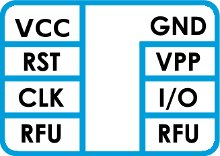
\includegraphics[scale=.3]{Imagenes/sc1.jpg} 
  \end{center}
  \caption{Tarjeta de contacto}\label{Fig:SC_c} 
\end{figure}

La serie de estándares ISO/IEC 7816 e ISO/IEC 7810 definen:

\begin{itemize}
\item La forma física (parte 1). 
\item La posición de las formas de los conectores eléctricos (parte 2). 
\item Las características eléctricas (parte 3). 
\item Los protocolos de comunicación (parte 3).
\item El formato de los comandos (ADPU's) enviados a la tarjeta y las respuestas retornadas por la misma (parte 3).
\item La dureza de la tarjeta.
\item La funcionalidad.
\end{itemize}


\bigskip
\leftline{bf{Tarjetas Inteligentes sin Contacto}}

El segundo tipo es la tarjeta inteligente sin contacto, RFID,  en el cual el chip se comunica con el lector de tarjetas mediante acoplamiento magnético a una tasa de transferencia de 106 a 848 Kbits/s.
El estándar de comunicación de tarjetas inteligentes sin contacto es el ISO/IEC 14443. Define dos tipos de tarjetas sin contacto (A y B), permitidos para distancias de comunicación de hasta 10cm. Las más abundantes son las tarjetas de la familia MIFARE de Philips, las cuales representan a la ISO/IEC 14443-A.
Las tarjetas inteligentes sin contacto son una evolución de la tecnología usada desde hace años por los RFID (identificación por radio frecuencia), añadiéndoles dispositivos que los chip RFID no suelen incluir, como memoria de escritura o microcontroladores.

\bigskip
Tarjetas híbridas y duales

\bigskip
Una tarjeta híbrida es una tarjeta sin contacto (contactless) a la cual se le agrega un segundo chip de contacto. Ambos chips pueden ser chips microprocesadores o simples chips de memoria. El chip sin contacto es generalmente usado en aplicaciones que requieren transacciones rápidas. Por ejemplo el transporte, mientras que el chip de contacto es generalmente utilizado en aplicaciones que requieren de alta seguridad como las bancarias.


\bigskip
Seguridad

La seguridad es una de las propiedades más importantes de las tarjetas inteligentes y se aplica a múltiples niveles y con distintos mecanismos. Cada fichero lleva asociadas unas condiciones de acceso y deben ser satisfechas antes de ejecutar un comando sobre ese fichero.

\bigskip
En el momento de personalización de la tarjeta (durante su fabricación) se puede indicar que mecanismos de seguridad se aplican a los ficheros. Normalmente se definirán:

\begin{itemize}
\item Ficheros de acceso libre.
\item Ficheros protegidos por claves: Pueden definirse varias claves con distintos propósitos. Normalmente se definen claves para proteger la escritura de algunos ficheros y claves específicas para los comandos de consumo y carga de las aplicaciones de monedero electrónico. De ese modo la aplicación que intente ejecutar comandos sobre ficheros protegidos tendrá que negociar previamente con la tarjeta la clave oportuna. 
\item Ficheros protegidos por PIN: El PIN es un número secreto que va almacenado en un fichero protegido y que es solicitado al usuario para acceder a este tipo de ficheros protegidos. Cuando el usuario lo introduce y el programa se lo pasa a la operación que va a abrir el fichero en cuestión, el sistema valida que el PIN sea correcto para dar acceso al fichero. 
\end{itemize}

La negociación de claves se realiza habitualmente apoyándose en un Módulo SAM, que no deja de ser otra tarjeta inteligente en formato ID-000 alojada en un lector interno propio dentro de la carcasa del lector principal o del TPV(Terminal de Punto de Venta) y que contiene aplicaciones criptográficas que permiten negociar las claves oportunas con la tarjeta inteligente del usuario. Operando de este modo se está autenticando el lector, la tarjeta y el módulo SAM involucrados en cada operación.


\bigskip
Programación de aplicaciones para los sistemas en los que se utiliza la tarjeta

\bigskip
Existen varias API de programación estandarizadas para comunicarse con los lectores de tarjetas inteligentes desde un computador. Las principales son:

\begin{itemize}
\item PC/SC (Personal Computer/Smart Card). El proyecto MUSCLE proporciona una implementación casi completa de esta especificación para los sistemas operativos GNU Linux-UNIX. 
\item OCF (OpenCard Framework), especificado por el grupo de empresas OpenCard. Este entorno intenta proporcionar un diseño orientado a objetos fácilmente extensible y modular. El consorcio OpenCard publica el API y proporciona una implementación de referencia en Java. Existe un adaptador para que OCF trabaje sobre PC/SC. 
\end{itemize}


En ambos casos, el modelo de programación que utilizan las tarjetas inteligentes está basado en protocolos de petición-respuesta. La tarjeta (su software) expone una serie de comandos que pueden ser invocados. Estos comandos interactúan con los ficheros que subyacen a cada aplicación de la tarjeta y proporcionan un resultado. Desde el terminal se invocan estos comandos a través de cualquiera de las API antes descritas componiendo un APDU (Application Protocol Data Unit - comandos con parámetros) que son enviados a la tarjeta para que ésta responda.


\section{ISO 14443}

ISO 14443 es un estándar internacional relacionado con las tarjetas de identificación electrónicas, en especial las smart cards, gestionado conjuntamente por la Organización Internacional de Normalización (ISO) y la Comisión Electrotécnica Internacional (IEC).
Este estándar define una tarjeta de proximidad utilizada para identificación y pagos que por lo general utiliza el formato de tarjeta de crédito definida por ISO 7816 - ID 1 (aunque otros formatos son posibles).
El sistema RFID utiliza un lector con un microcontrolador o ASIC y una antena que opera a 13,56MHz (frecuencia RFID). El lector mantiene a su alrededor un campo electromagnético de modo que al acercarse una tarjeta al campo, ésta se alimenta eléctricamente de esta energía inducida y puede establecerse la comunicación lector-tarjeta.

\begin{figure}[H]
\centering
  \begin{center}
  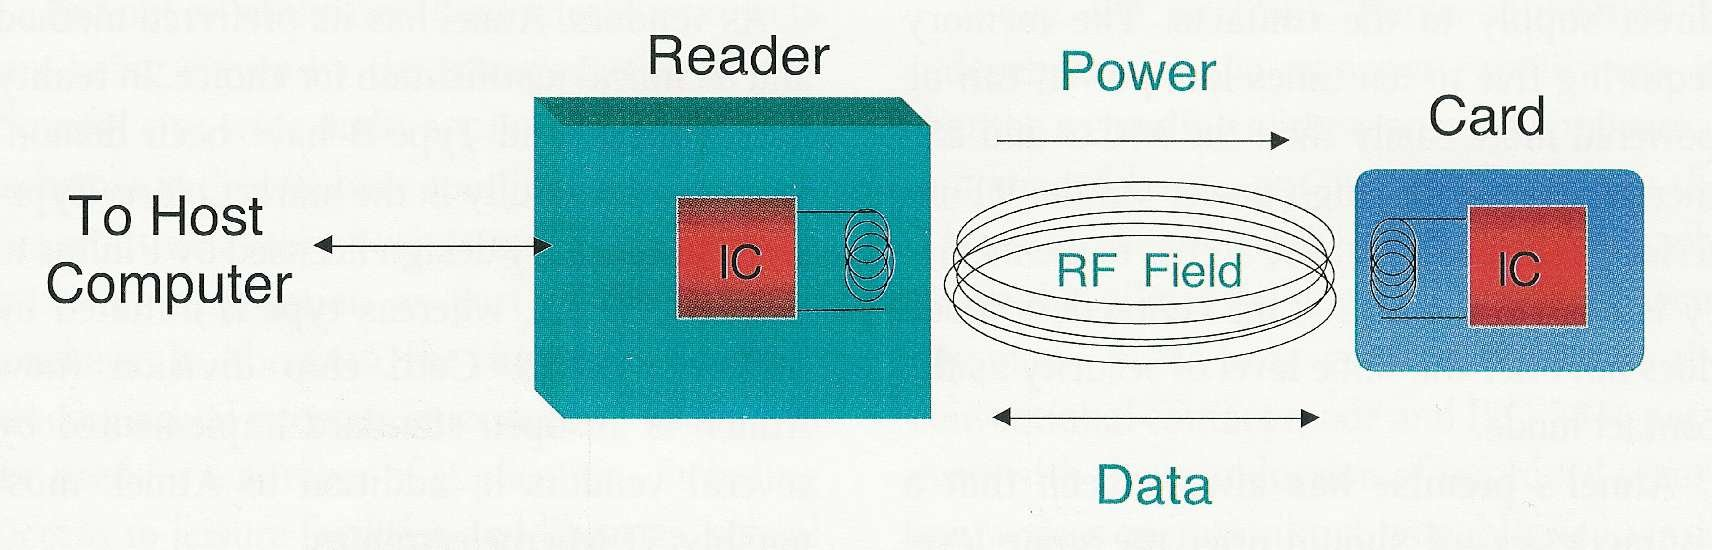
\includegraphics[scale=.2]{Imagenes/sc2.jpg} 
  \end{center}
  \caption{Acoplamiento entre lector y tarjeta}\label{Fig:RFID3} 
\end{figure}

El estándar ISO 14443 consta de cuatro partes y se describen dos tipos de tarjetas: tipo A y tipo B. Las principales diferencias entre estos tipos está en los métodos de modulación, codificación de los planes (parte2) y el protocolo de inicialización de los procedimientos (parte3). Las tarjetas de ambos tipos (A y B) utilizan el mismo protocolo de alto nivel (llamado T=CL) que se describe en la parte4. El protocolo T=CL especifica los bloques de datos y los mecanismos de intercambio:

\begin{itemize}
\item[1.] Bloque de datos de encadenamiento.
\item[2.] Tiempo de espera de extensión.
\item[3.] Múltiple activación.
\end{itemize}

Las tarjetas Mifare cumplen con las partes 1, 2 y 3 de tipo A de la especificación ISO/IEC 14443.


\section{Mifare}

Mifare es la tecnología de smart card sin contacto más ampliamente usada en el mundo. Es equivalente a las 3 primeras partes de la norma ISO 14443 Tipo A. La distancia típica de lectura es de hasta 10 cm, depende de la potencia del lector y factores del entorno, existiendo lectores de mayor y menor alcance.
La tecnología Mifare es económica y rápida, razón por la cual es la más usada a nivel mundial hoy día.


\subsection{Operación}

Las tarjetas Mifare son tarjetas de memoria protegida. Están divididas en sectores que a su vez son subdivididos en bloques y poseen mecanismos de seguridad para el control de acceso. Su capacidad de cómputo no permite realizar operaciones criptográficas o de autenticación mutua de alto nivel, estando principalmente destinadas a monederos electrónicos simples, control de acceso, tarjetas de identidad corporativas, tarjetas de transporte urbano o para ticketing.
Cada sector se divide en cuatro bloques, de los cuales tres pueden contener información del usuario, y el cuarto, llamado trailer, contiene elementos de seguridad. La información es almacenada sin un  formato pre establecido, y se puede modificar con comandos simples de lectura y escritura. Mifare provee un formato especial llamado “bloque de valor”(value block); los bloques que tienen información guardada en este formato se comportan de una forma diferente, incluyendo operaciones de incremento y descuento.
Los sectores utilizan dos claves de acceso llamadas 'A' y 'B'. Estas claves se almacenan en el cuarto bloque junto con los permisos de acceso a cada uno de los tres bloques que son parte del mismo sector. Estos permisos pueden ser: lectura, escritura, descuento o incremento (para bloques de valor).

\begin{figure}[H]
\centering
  \begin{center}
  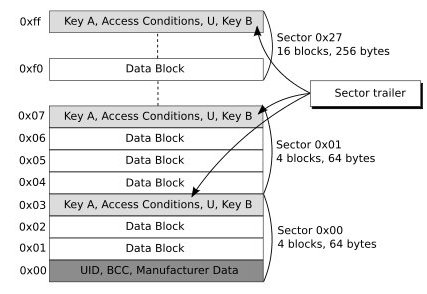
\includegraphics[scale=.6]{Imagenes/sc3.jpg} 
  \end{center}
  \caption{Mifare Classic de 4K}\label{Fig:MC_4K} 
\end{figure}

Una vez que se acerca la tarjeta a un lector, ésta se activa e inicia un proceso de intercambio con el lector para establecer una comunicación cifrada. Este proceso es igual con todas las tarjetas y está diseñado para proveer protección del canal(evitando que se espíe), y no para autenticar la tarjeta o el lector.
Previo a establecer un canal cifrado la tarjeta envía un código de identificación, mediante el algoritmo de anticolisión, que usualmente es el número de serie de la tarjeta, aunque la norma ISO 14443 indica que este número puede ser aleatorio. Con este número de identificación el lector está en condiciones de realizar cualquier operación en la tarjeta, previa autenticación con las claves de acceso en los respectivos sectores.
Se debe destacar que un sistema con claves diversificadas facilita el fortalecimiento de la seguridad, apoyada por una base de datos que pueda monitorear los aumentos de los saldos y demás estrategias operativas y finalmente la autenticación remota por SAM, no todos los sistemas poseen esto.

\bigskip
Variantes

\begin{itemize}
\item Mifare Classic. Son fundamentalmente de los dispositivos de almacenamiento de memoria. Existen tarjetas de 1Kb y de 4Kb. La Mifare Standard de 1KB ofrece unos 768 bytes de almacenamiento de datos, dividida en 16 sectores. La Mifare Standard de 4k ofrece 3 KB dividido en 64 sectores. 
\item Mifare Ultralight. Es semejante a la classic, pero sólo tiene 512 bits de memoria (es decir 64 octetos), sin seguridad. Esta tarjeta es muy barata así que se utiliza a menudo de forma desechable. 
\item Mifare T = CL. Bajo esta denominación se encuadran las tarjetas Mifare ProX y SmartMX. Son tarjetas con microprocesador que incorporan un sistema operativo de tarjeta (Card Operating System - COS) y aplicaciones desarrolladas específicamente para ser ejecutadas en la tarjeta. Estas tarjetas son capaces de ejecutar operaciones complejas de forma rápida y segura, igual que las tarjetas con contactos ISO 7816. 
\item Mifare DESFire. Esta tarjeta es una versión especial de Philips SmartMX. Se vende con un software de propósito general incorporado (el sistema operativo DESFire), que ofrece más o menos las mismas funciones que Mifare Standard (4kB de almacenamiento de datos dividido en 16 bloques), pero con una mayor flexibilidad, una mayor seguridad (triple DES), y con mayor rapidez (protocolo T=CL). 
\item Mifare DESFire EV1. Es la primera evolución de Mifare DESFire, compatible con la versión anterior, pero aún más segura, alcanzando la certificación EAL 4.
\end{itemize}